\usetikzlibrary{positioning,arrows.meta,shadows}
\usepackage{xifthen}
% definitions for list
\newcommand\boxsize{6mm}
\tikzset
  {cell/.style=
    {inner sep=0pt, minimum width=\boxsize, minimum height=\boxsize, fill=white},
   ptr/.style={Circle-stealth, shorten <=-1.5pt}
  }
\newcommand\pointer[3][] {
  \node[draw,cell,#1] (#2) {};
  \ifthenelse{\isempty{#3}}
    {\draw (#2.south west)--(#2.north east) (#2.north west)--(#2.south east);}
    {\draw[ptr] (#2.center)--(#3);}
}

\newcommand\element[4][] {
  \node[draw, cell, #1] (#2) {#3};
  \node[draw, cell, xshift=\boxsize] (#2ptr) at (#2) {};
  \ifthenelse{\isempty{#4}}
    {\draw (#2ptr.south west)--(#2ptr.north east) (#2ptr.north west)--(#2ptr.south east);}
    {\draw[ptr] (#2ptr.center)--(#4);}
}

\begin{document}

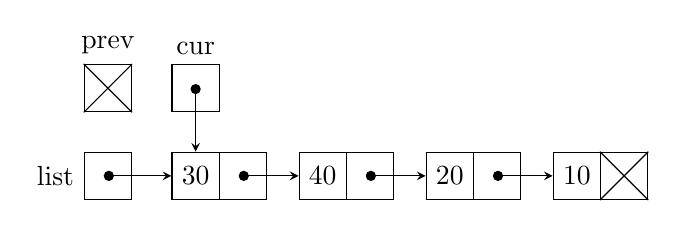
\begin{tikzpicture}
  \element{e1}{10}{}
  \element[left=of e1]{e2}{20}{e1}
  \element[left=of e2]{e3}{40}{e2}
  \element[left=of e3]{e4}{30}{e3}
  \pointer[left=5mm of e4, label=left:list]{list}{e4}
  \pointer[above=5mm of e4, label=above:cur]{cur}{e4}
  \pointer[above=5mm of list, label=above:prev]{prev}{}
\end{tikzpicture}

\end{document}
